% ============================================================================
% CHAPITRE 3 — Missions et travaux réalisés
% ============================================================================
\openchapter{Missions et travaux réalisés}

\section{Introduction}

Ce chapitre présente la spécification fonctionnelle du système, les acteurs
identifiés et leurs rôles, la structure des données manipulées, l'architecture
technique retenue, l'environnement de développement, le détail des
fonctionnalités implémentées, ainsi que les interfaces développées pour
chaque profil d'utilisateur.

\section{Spécification fonctionnelle}

À partir du cahier des charges du stage, le système doit permettre :

\begin{itemize}
  \item la \textbf{gestion des adhérents} : création d'un profil adhérent,
    consultation et mise à jour de ses coordonnées, suppression ;
  \item la \textbf{gestion des cotisations annuelles} : enregistrement d'un
    paiement de cotisation avec son reçu, vérification par un rôle financier
    du bureau, suivi d'une cotisation \emph{due} par adhérent et par année
    (montant dû, montant payé, solde, statut), avec génération automatique
    des cotisations et détection des retards ;
  \item la \textbf{gestion des projets associatifs} : création d'un projet,
    constitution d'un comité dédié, suivi de son cycle de vie jusqu'à sa
    clôture ou son annulation ;
  \item les \textbf{comités par projet} : chaque comité regroupe des membres
    avec un rôle propre au projet (président de comité, trésorier,
    secrétaire, membre), indépendant du rôle global de la personne dans
    l'association, et saisit les opérations financières du projet selon ce
    rôle ;
  \item le \textbf{workflow des dons et des dépenses} avec approbation :
    toute entrée ou sortie d'argent sur un projet passe par un circuit
    brouillon~$\rightarrow$~soumis~$\rightarrow$~approuvé ou rejeté, avec
    justificatif obligatoire (reçu, facture, photo de chèque ou d'ordre de
    virement) ;
  \item les \textbf{rapports de clôture} : à la fin d'un projet, un rapport
    PDF récapitulant les entrées, les dépenses et les justificatifs est
    généré automatiquement, et un rapport association-wide (adhérents,
    cotisations, projets, cotisations dues) est disponible en PDF et Excel
    à tout moment pour le bureau ;
  \item la \textbf{consultation en libre-service}, pour chaque adhérent, de
    son propre historique : cotisations, dons effectués, solde dû.
\end{itemize}

\section{Identification des acteurs et rôles}

Le cahier des charges distingue le \emph{rôle global} d'une personne dans
l'association (président, vice-président, trésorier, vice-trésorier,
secrétaire général, vice-secrétaire général, conseiller, ou simple adhérent)
de son éventuel \emph{rôle dans un comité de projet} (président de comité,
trésorier de comité, secrétaire, membre) : les membres du bureau de
l'association sont eux-mêmes des adhérents, et un adhérent sans rôle global
particulier peut être trésorier d'un comité de projet donné.


\begin{figure}[H]
    \centering
    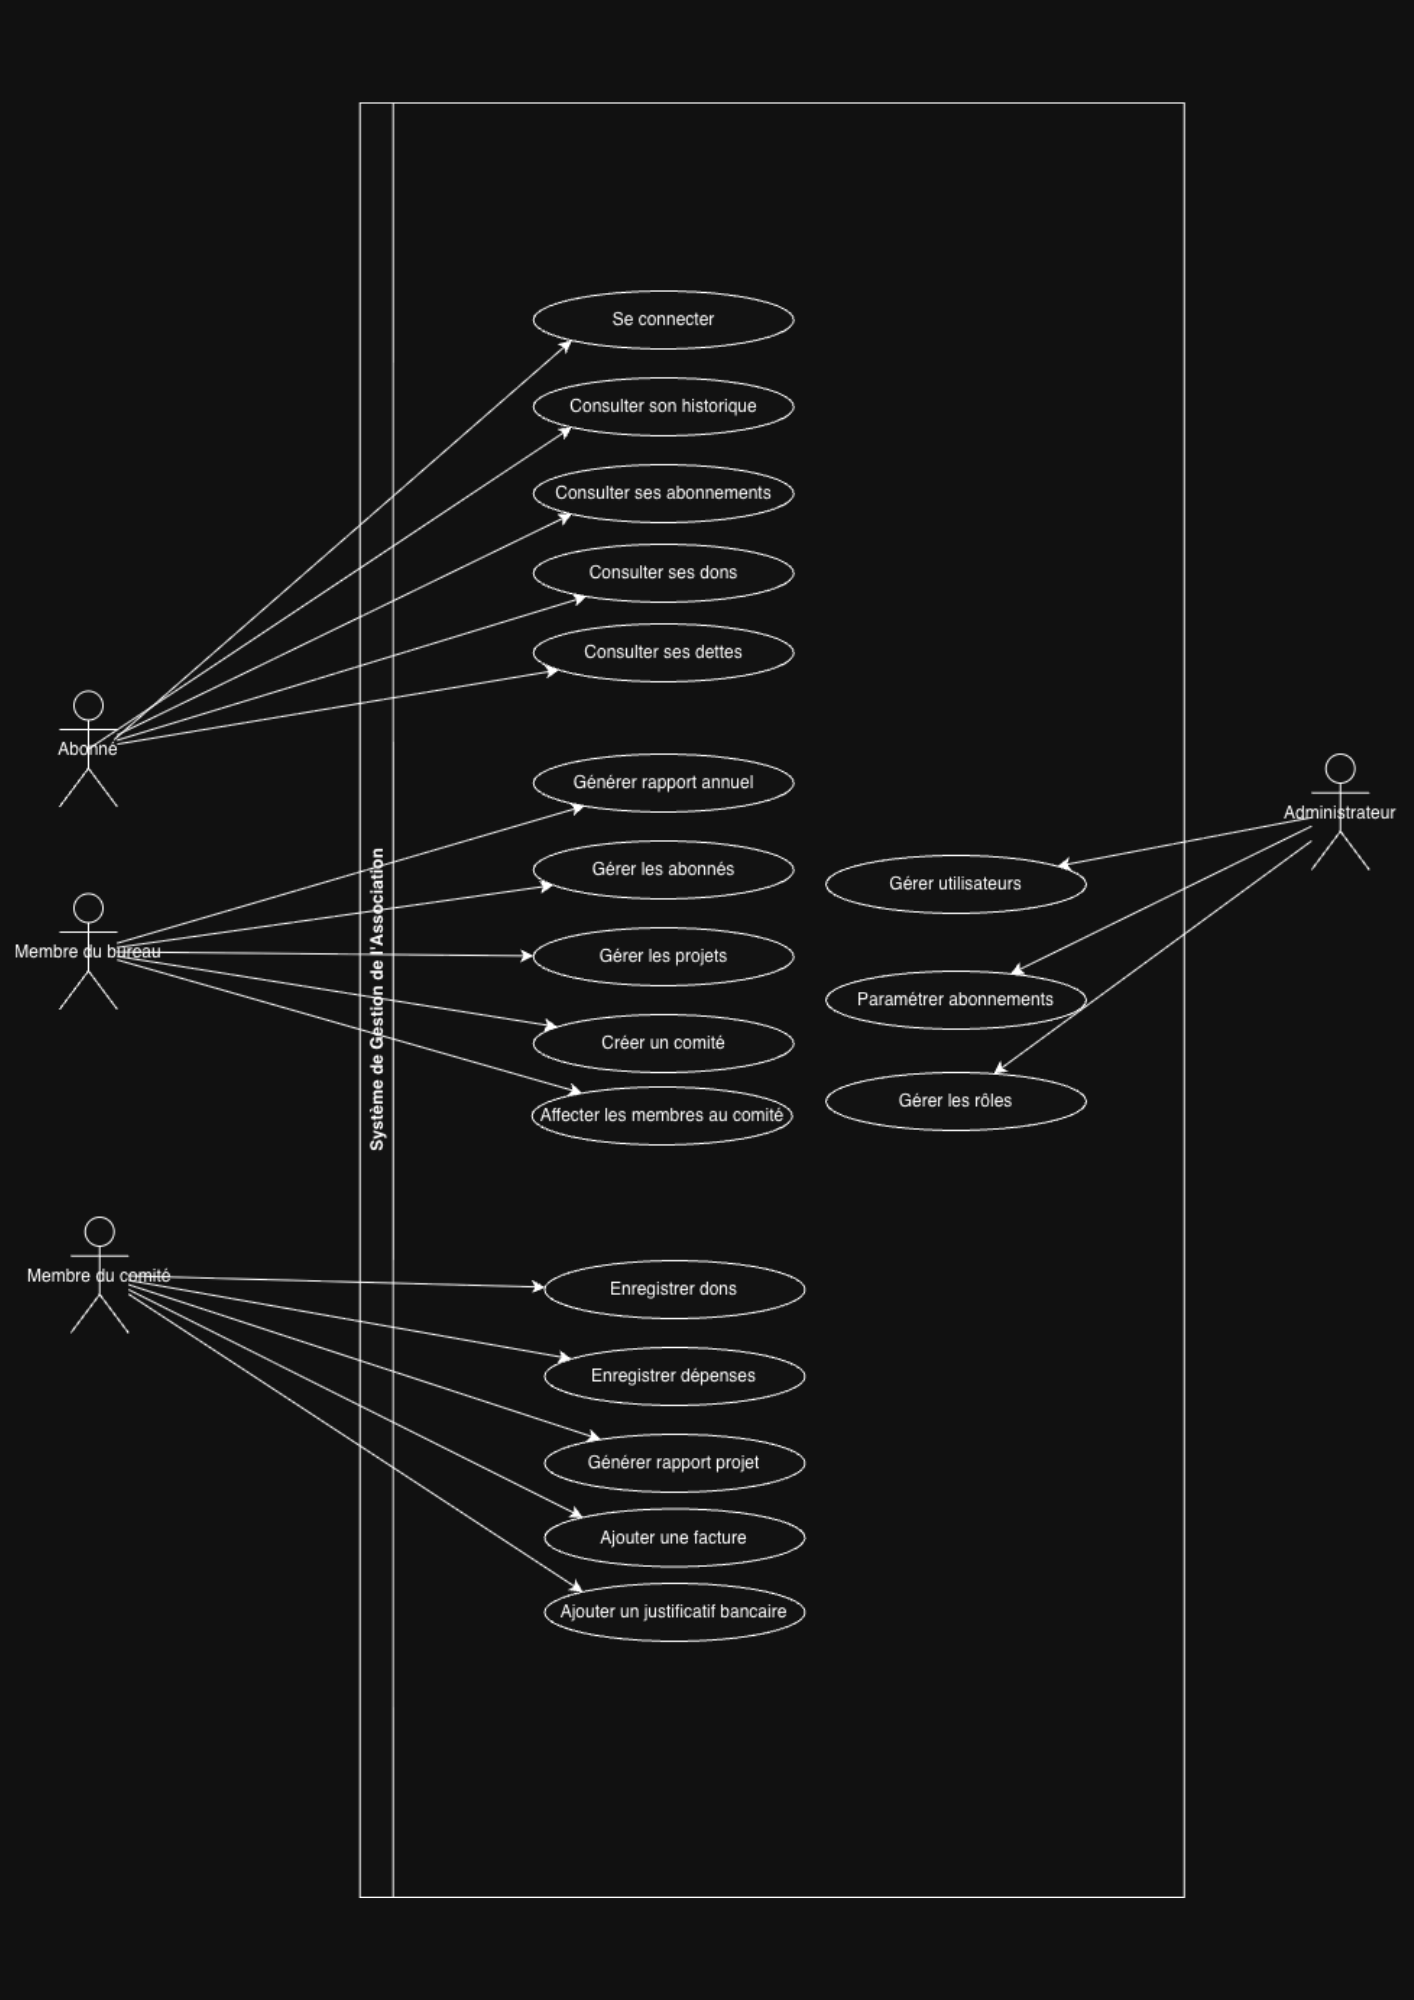
\includegraphics[width=\textwidth]{use-case.png}
    \caption{Diagramme de cas d'utilisation}
    \label{fig:use-case}
\end{figure}


Le détail complet des droits par rôle global (adhérents, cotisations, dues,
projets, dons, dépenses) figure dans la matrice de l'Annexe~B.

\section{Structure des données}

La figure~\ref{fig:classes} présente une vue simplifiée des principales
entités manipulées par le système et de leurs relations. \texttt{Member}
représente un adhérent (lié à un compte \texttt{User} pour l'authentification,
non représenté ici) ; \texttt{Due} porte le montant dû par un adhérent pour
une année donnée, réglé par une ou plusieurs \texttt{Subscription} (paiements
de cotisation) ; \texttt{Project} centralise le cycle de vie d'un projet, ses
\texttt{Donation}, ses \texttt{Expense} et les transferts de fonds
(\texttt{ProjectFundAllocation}) qui lui sont alloués ; \texttt{CommitteeAssignment}
est l'historique, jamais supprimé, des rôles tenus par un adhérent au sein du
comité d'un projet ; \texttt{ProjectReport} porte le rapport de clôture
généré à la fin d'un projet ; \texttt{Notification} peut être rattachée à
n'importe laquelle des autres entités (relation polymorphique).

\begin{figure}[htbp]
  \centering
  \begin{tikzpicture}[node distance=0.9cm and 0.9cm, every node/.style={font=\scriptsize}]
    \node[entitybox] (member) {\textbf{Member}\\ user\_id, phone, address};
    \node[entitybox, right=2.6cm of member] (project) {\textbf{Project}\\ name, budget, status, phase};

    \node[entitybox, below=of member] (subscription) {\textbf{Subscription}\\ member\_id, due\_id, amount, status};
    \node[entitybox, left=1.1cm of subscription] (due) {\textbf{Due}\\ member\_id, year, amount\_due,\\ balance, status};

    \node[entitybox, below=of project] (committee) {\textbf{CommitteeAssignment}\\ project\_id, member\_id,\\ committee\_role, action};
    \node[entitybox, right=1.1cm of committee] (allocation) {\textbf{ProjectFundAllocation}\\ project\_id, amount, allocation\_date};

    \node[entitybox, below=1.6cm of subscription] (donation) {\textbf{Donation}\\ member\_id, project\_id,\\ amount, status};
    \node[entitybox, right=1.1cm of donation] (expense) {\textbf{Expense}\\ project\_id, amount,\\ status};
    \node[entitybox, right=1.1cm of expense] (report) {\textbf{ProjectReport}\\ project\_id, file\_path, summary};

    \node[entitybox, below=2.4cm of project] (notification) {\textbf{Notification}\\ user\_id, type,\\ subject\_type, subject\_id};

    \draw[bluearrow] (member.east) -- (subscription.north);
    \draw[bluearrow] (member.west) .. controls +(-0.8,0) and +(-0.8,0) .. (due.north);
    \draw[bluearrow] (subscription.west) -- node[above,font=\tiny]{règle} (due.east);
    \draw[bluearrow] (member.south) .. controls +(0,-2) and +(2,2.4) .. (donation.north);
    \draw[bluearrow] (member.east) .. controls +(3.2,-1) and +(3.4,4) .. (committee.north east);

    \draw[bluearrow] (project.south) -- (committee.north);
    \draw[bluearrow] (project.east) .. controls +(1,-1) and +(0,1.4) .. (allocation.north);
    \draw[bluearrow] (project.south) .. controls +(0,-2.2) and +(2,3.4) .. (donation.north east);
    \draw[bluearrow] (project.south) .. controls +(1,-2.6) and +(0,2.4) .. (expense.north);
    \draw[bluearrow] (project.south) .. controls +(2,-2.8) and +(0,2.6) .. (report.north);
    \draw[bluearrow] (project.south) .. controls +(-1.4,-4.6) and +(1,3.4) .. (notification.east);
    \draw[bluearrow] (donation.south) .. controls +(0,-1) and +(-1,1) .. (notification.north west);
  \end{tikzpicture}
  \caption{Diagramme de classes simplifié du système.}
  \label{fig:classes}
\end{figure}

\section{Architecture technique}

Le système est bâti selon une architecture web classique en trois niveaux :
une interface web (React) qui consomme une API REST (Laravel), elle-même
adossée à une base de données relationnelle (MySQL) et à un espace de
stockage de fichiers pour les justificatifs. La figure~\ref{fig:architecture}
résume cette organisation.

\begin{figure}[htbp]
  \centering
  \begin{tikzpicture}[node distance=0.7cm]
    \node[archbox, text width=9.5cm, minimum height=1.6cm] (front)
      {\textbf{Interface web} --- React~19 + Vite, Tailwind~CSS,\\ Recharts, TomTom Maps SDK, ExcelJS};
    \node[archbox, below=of front, text width=9.5cm, minimum height=2.1cm] (api)
      {\textbf{API REST} --- Laravel~13\\ Authentification par jeton (Sanctum) $\cdot$ Rôles et permissions (Spatie)\\ Policies par ressource $\cdot$ Génération PDF (dompdf) $\cdot$ Export Excel};
    \node[archbox, below=of api, text width=4.5cm, minimum height=1.4cm] (db)
      {\textbf{Base de données}\\ MySQL};
    \node[archbox, right=1cm of db, text width=4.5cm, minimum height=1.4cm] (storage)
      {\textbf{Stockage fichiers}\\ Reçus, factures, rapports PDF};

    \draw[bluearrow] (front.south) -- node[right,font=\scriptsize]{HTTP / JSON} (api.north);
    \draw[bluearrow] (api.south) -- (db.north -| api.south);
    \draw[bluearrow] (api.south) -- (storage.north -| api.south);
  \end{tikzpicture}
  \caption{Architecture générale de la plateforme.}
  \label{fig:architecture}
\end{figure}

\section{Environnement de développement}

Le tableau~\ref{tab:outils} présente les principaux outils et technologies
utilisés pour la réalisation du projet.

\begin{center}
\begin{longtable}{@{}p{2.6cm}p{11.5cm}@{}}
\toprule
\textbf{Outil} & \textbf{Rôle dans le projet} \\
\midrule
\endhead
\colorbox{lightblue}{\parbox[c][0.9cm][c]{2.3cm}{\centering\bfseries React}} &
  Bibliothèque JavaScript utilisée pour l'interface web : tableau de bord,
  pages de gestion des adhérents, des projets, des finances et des rapports,
  toutes consommant l'API REST du backend. \\[0.4cm]
\colorbox{lightblue}{\parbox[c][0.9cm][c]{2.3cm}{\centering\bfseries Laravel}} &
  Framework PHP utilisé pour l'API REST : routage, validation des requêtes,
  authentification, autorisation et accès aux données. \\[0.4cm]
\colorbox{lightblue}{\parbox[c][0.9cm][c]{2.3cm}{\centering\bfseries MySQL}} &
  Système de gestion de base de données relationnelle stockant les
  adhérents, cotisations, projets, dons, dépenses et journaux d'activité. \\[0.4cm]
\colorbox{lightblue}{\parbox[c][0.9cm][c]{2.3cm}{\centering\bfseries Tailwind CSS}} &
  Framework CSS utilitaire pour la mise en forme de l'interface web. \\[0.4cm]
\colorbox{lightblue}{\parbox[c][0.9cm][c]{2.3cm}{\centering\bfseries Sanctum}} &
  Extension Laravel gérant l'authentification par jeton (bureau et portail
  adhérent), utilisée pour sécuriser chaque appel à l'API. \\[0.4cm]
\colorbox{lightblue}{\parbox[c][0.9cm][c]{2.3cm}{\centering\bfseries Spatie Permission}} &
  Bibliothèque de gestion des rôles et permissions, à la base du contrôle
  d'accès par rôle global décrit à la section~III. \\[0.4cm]
\colorbox{lightblue}{\parbox[c][0.9cm][c]{2.3cm}{\centering\bfseries dompdf}} &
  Génération des rapports PDF (rapport de clôture de projet, rapports
  association, reçus). \\[0.4cm]
\colorbox{lightblue}{\parbox[c][0.9cm][c]{2.3cm}{\centering\bfseries Maatwebsite Excel}} &
  Export des rapports association (adhérents, cotisations, projets, dues)
  au format Excel. \\[0.4cm]
\colorbox{lightblue}{\parbox[c][0.9cm][c]{2.3cm}{\centering\bfseries TomTom Maps SDK}} &
  Sélection et affichage de la localisation géographique d'un projet sur une
  carte interactive. \\
\bottomrule
\caption{Principaux outils et technologies utilisés pour le développement.}
\label{tab:outils}
\end{longtable}
\end{center}

\section{Fonctionnalités implémentées}

\subsection{Cycle de vie des projets}

Un projet suit un cycle de vie à cinq états administratifs, illustré à la
figure~\ref{fig:lifecycle}. Le passage de \emph{brouillon} à \emph{comité
constitué} se produit automatiquement dès qu'un premier membre est affecté au
comité du projet ; le passage à \emph{financement réuni} se produit
automatiquement dès la première allocation de fonds. Le démarrage
(\emph{actif}) et la clôture (\emph{terminé}) sont des actions explicites du
président ou du président de comité. Un projet peut être annulé depuis
n'importe quel état non terminal. Une fois \emph{terminé} ou \emph{annulé},
un projet devient définitivement en lecture seule et son comité est dissous.

\begin{figure}[htbp]
  \centering
  \begin{tikzpicture}[node distance=1.6cm, every node/.style={font=\small}]
    \node[statebox] (draft) {Brouillon};
    \node[statebox, right=of draft] (committee) {Comité constitué};
    \node[statebox, right=of committee] (funding) {Financement réuni};
    \node[statebox, right=of funding] (active) {Actif};
    \node[statebox, right=of active] (done) {Terminé};
    \node[statebox, below=1.2cm of active] (cancelled) {Annulé};

    \draw[bluearrow] (draft) -- node[above,font=\scriptsize]{1\textsuperscript{er} membre affecté} (committee);
    \draw[bluearrow] (committee) -- node[above,font=\scriptsize]{1\textsuperscript{re} allocation} (funding);
    \draw[bluearrow] (funding) -- node[above,font=\scriptsize]{démarrage} (active);
    \draw[bluearrow] (active) -- node[above,font=\scriptsize]{clôture} (done);
    \draw[bluearrow] (draft.south) -- (cancelled.west);
    \draw[bluearrow] (committee.south) -- (cancelled.north west);
    \draw[bluearrow] (funding.south) -- (cancelled.north);
    \draw[bluearrow] (active.south) -- (cancelled.north);
  \end{tikzpicture}
  \caption{Cycle de vie administratif d'un projet.}
  \label{fig:lifecycle}
\end{figure}

Un second axe, indépendant, suit l'avancement \emph{réel} du projet
(\emph{planification} $\rightarrow$ \emph{préparation} $\rightarrow$ \emph{en
cours} $\rightarrow$ \emph{finition} $\rightarrow$ \emph{terminé}) : le
président de comité soumet une demande de passage à l'étape suivante, avec
justificatifs, que le président ou le vice-président approuve ou rejette.
Cet avancement ne peut jamais être modifié directement, ni sauter une étape.

\subsection{Workflow d'approbation des dons et des dépenses}

Chaque don et chaque dépense saisi par un comité suit le même circuit
d'approbation (figure~\ref{fig:approbation}) : un membre habilité du comité
(président ou trésorier de comité) crée l'enregistrement à l'état
\emph{brouillon}, le complète avec son justificatif (reçu ou facture) puis le
soumet. Seul un rôle financier du bureau (président, trésorier ou
vice-trésorier) peut ensuite l'approuver ou le rejeter ; la personne qui a
saisi l'opération ne peut jamais approuver sa propre saisie. Un rejet précise
son motif et son type (justificatif à remplacer, ou détails erronés) : dans
le premier cas, le comité peut corriger le justificatif et resoumettre le
même enregistrement ; dans le second, l'enregistrement reste figé et une
nouvelle saisie doit être créée. Pour une dépense uniquement, une fois
approuvée, elle peut être marquée \emph{payée} — un état terminal.

\begin{figure}[htbp]
  \centering
  \begin{tikzpicture}[node distance=1.7cm, every node/.style={font=\small}]
    \node[statebox] (draft) {Brouillon};
    \node[statebox, right=of draft] (pending) {Soumis};
    \node[statebox, above right=0.9cm and 1.7cm of pending] (approved) {Approuvé};
    \node[statebox, below right=0.9cm and 1.7cm of pending] (rejected) {Rejeté};
    \node[statebox, right=1.7cm of approved] (paid) {Payé\\ \scriptsize(dépenses)};

    \draw[bluearrow] (draft) -- (pending);
    \draw[bluearrow] (pending) -- (approved);
    \draw[bluearrow] (pending) -- (rejected);
    \draw[bluearrow] (approved) -- (paid);
    \draw[bluearrow] (rejected.north) to[out=110,in=-110] node[left,font=\scriptsize]{justificatif corrigé} (pending.south);
  \end{tikzpicture}
  \caption{Workflow d'approbation des dons et des dépenses.}
  \label{fig:approbation}
\end{figure}

\subsection{Système de comités et historique}

Avant tout projet, le bureau constitue un comité et affecte à chacun de ses
membres un rôle propre au projet (président de comité, trésorier, secrétaire
ou membre) — ce rôle détermine les droits de saisie décrits ci-dessus, quel
que soit le rôle global de la personne dans l'association. Chaque affectation,
remplacement, démission, retrait ou dissolution (à la clôture ou à
l'annulation du projet) est conservé dans un historique qui n'est jamais
purgé, consultable projet par projet, avec la date, l'auteur de l'action et
son motif.

\subsection{Cotisations annuelles et suivi des dues}

En complément du paiement d'une cotisation (\texttt{Subscription}), chaque
adhérent dispose d'un solde dû par année (\texttt{Due}) : montant dû, montant
réglé, solde restant, statut (en attente, partiel, payé, en retard, exonéré).
Ce solde est recalculé automatiquement à chaque paiement vérifié qui lui est
rattaché ; le rattachement lui-même est automatique dès la création d'un
paiement de cotisation. Une tâche planifiée génère les dues de l'année en
cours pour chaque adhérent et bascule au statut \emph{en retard} celles dont
l'échéance est dépassée sans solde nul. Un rôle financier du bureau peut, à
titre exceptionnel, exonérer une cotisation due.

\subsection{Rapports de clôture et rapports association}

À la clôture d'un projet, un rapport PDF est généré automatiquement :
total des dons, des dépenses, des fonds alloués, solde reversé à
l'association, accompagné du détail de chaque opération. Indépendamment,
le bureau dispose à tout moment de rapports association-wide (adhérents,
cotisations, projets, cotisations dues), téléchargeables en PDF ou au format
Excel.

\subsection{Journal d'activité}

Chaque création, modification ou action de workflow (soumission, approbation,
rejet, paiement) est journalisée automatiquement. Le journal est consultable
sous forme de recherche/filtre par utilisateur, projet, type d'entité, action
et période ; sa portée dépend du rôle du lecteur : le président, le
vice-président et le trésorier voient l'ensemble de l'activité, les autres
rôles du bureau ne voient que celle des projets auxquels ils sont affectés,
et un simple adhérent n'y a pas accès.

\subsection{Centre de notifications}

Chaque événement significatif (cotisation à vérifier, don ou dépense en
attente d'approbation, projet clôturé, cotisation en retard, affectation à un
comité, etc.) génère une notification pour les personnes concernées : la
personne à l'origine de l'action, les rôles habilités à la traiter, ou les
deux. Chaque notification renvoie directement vers l'écran concerné.

\subsection{Authentification}

Deux mécanismes d'authentification coexistent, contre le même jeton d'accès :
les membres du bureau se connectent par email et mot de passe ; un adhérent
se connecte par un code numérique à six chiffres (« passkey »), délivré
automatiquement par email la première fois que sa cotisation est vérifiée par
le bureau. Les deux profils accèdent ensuite au même tableau de bord, dont le
contenu s'adapte à leur rôle et à leurs éventuelles affectations de comité.

\section{Interfaces développées}

Cette section présente les principales interfaces développées, une par
profil d'utilisateur ou par domaine fonctionnel.

\subsection{Tableau de bord du président}

Le tableau de bord du président centralise les indicateurs clés de
l'association : fonds disponibles, cotisations, projets par état, comités,
ainsi que les listes d'approbations en attente.

\begin{figure}[htbp]
  \centering
  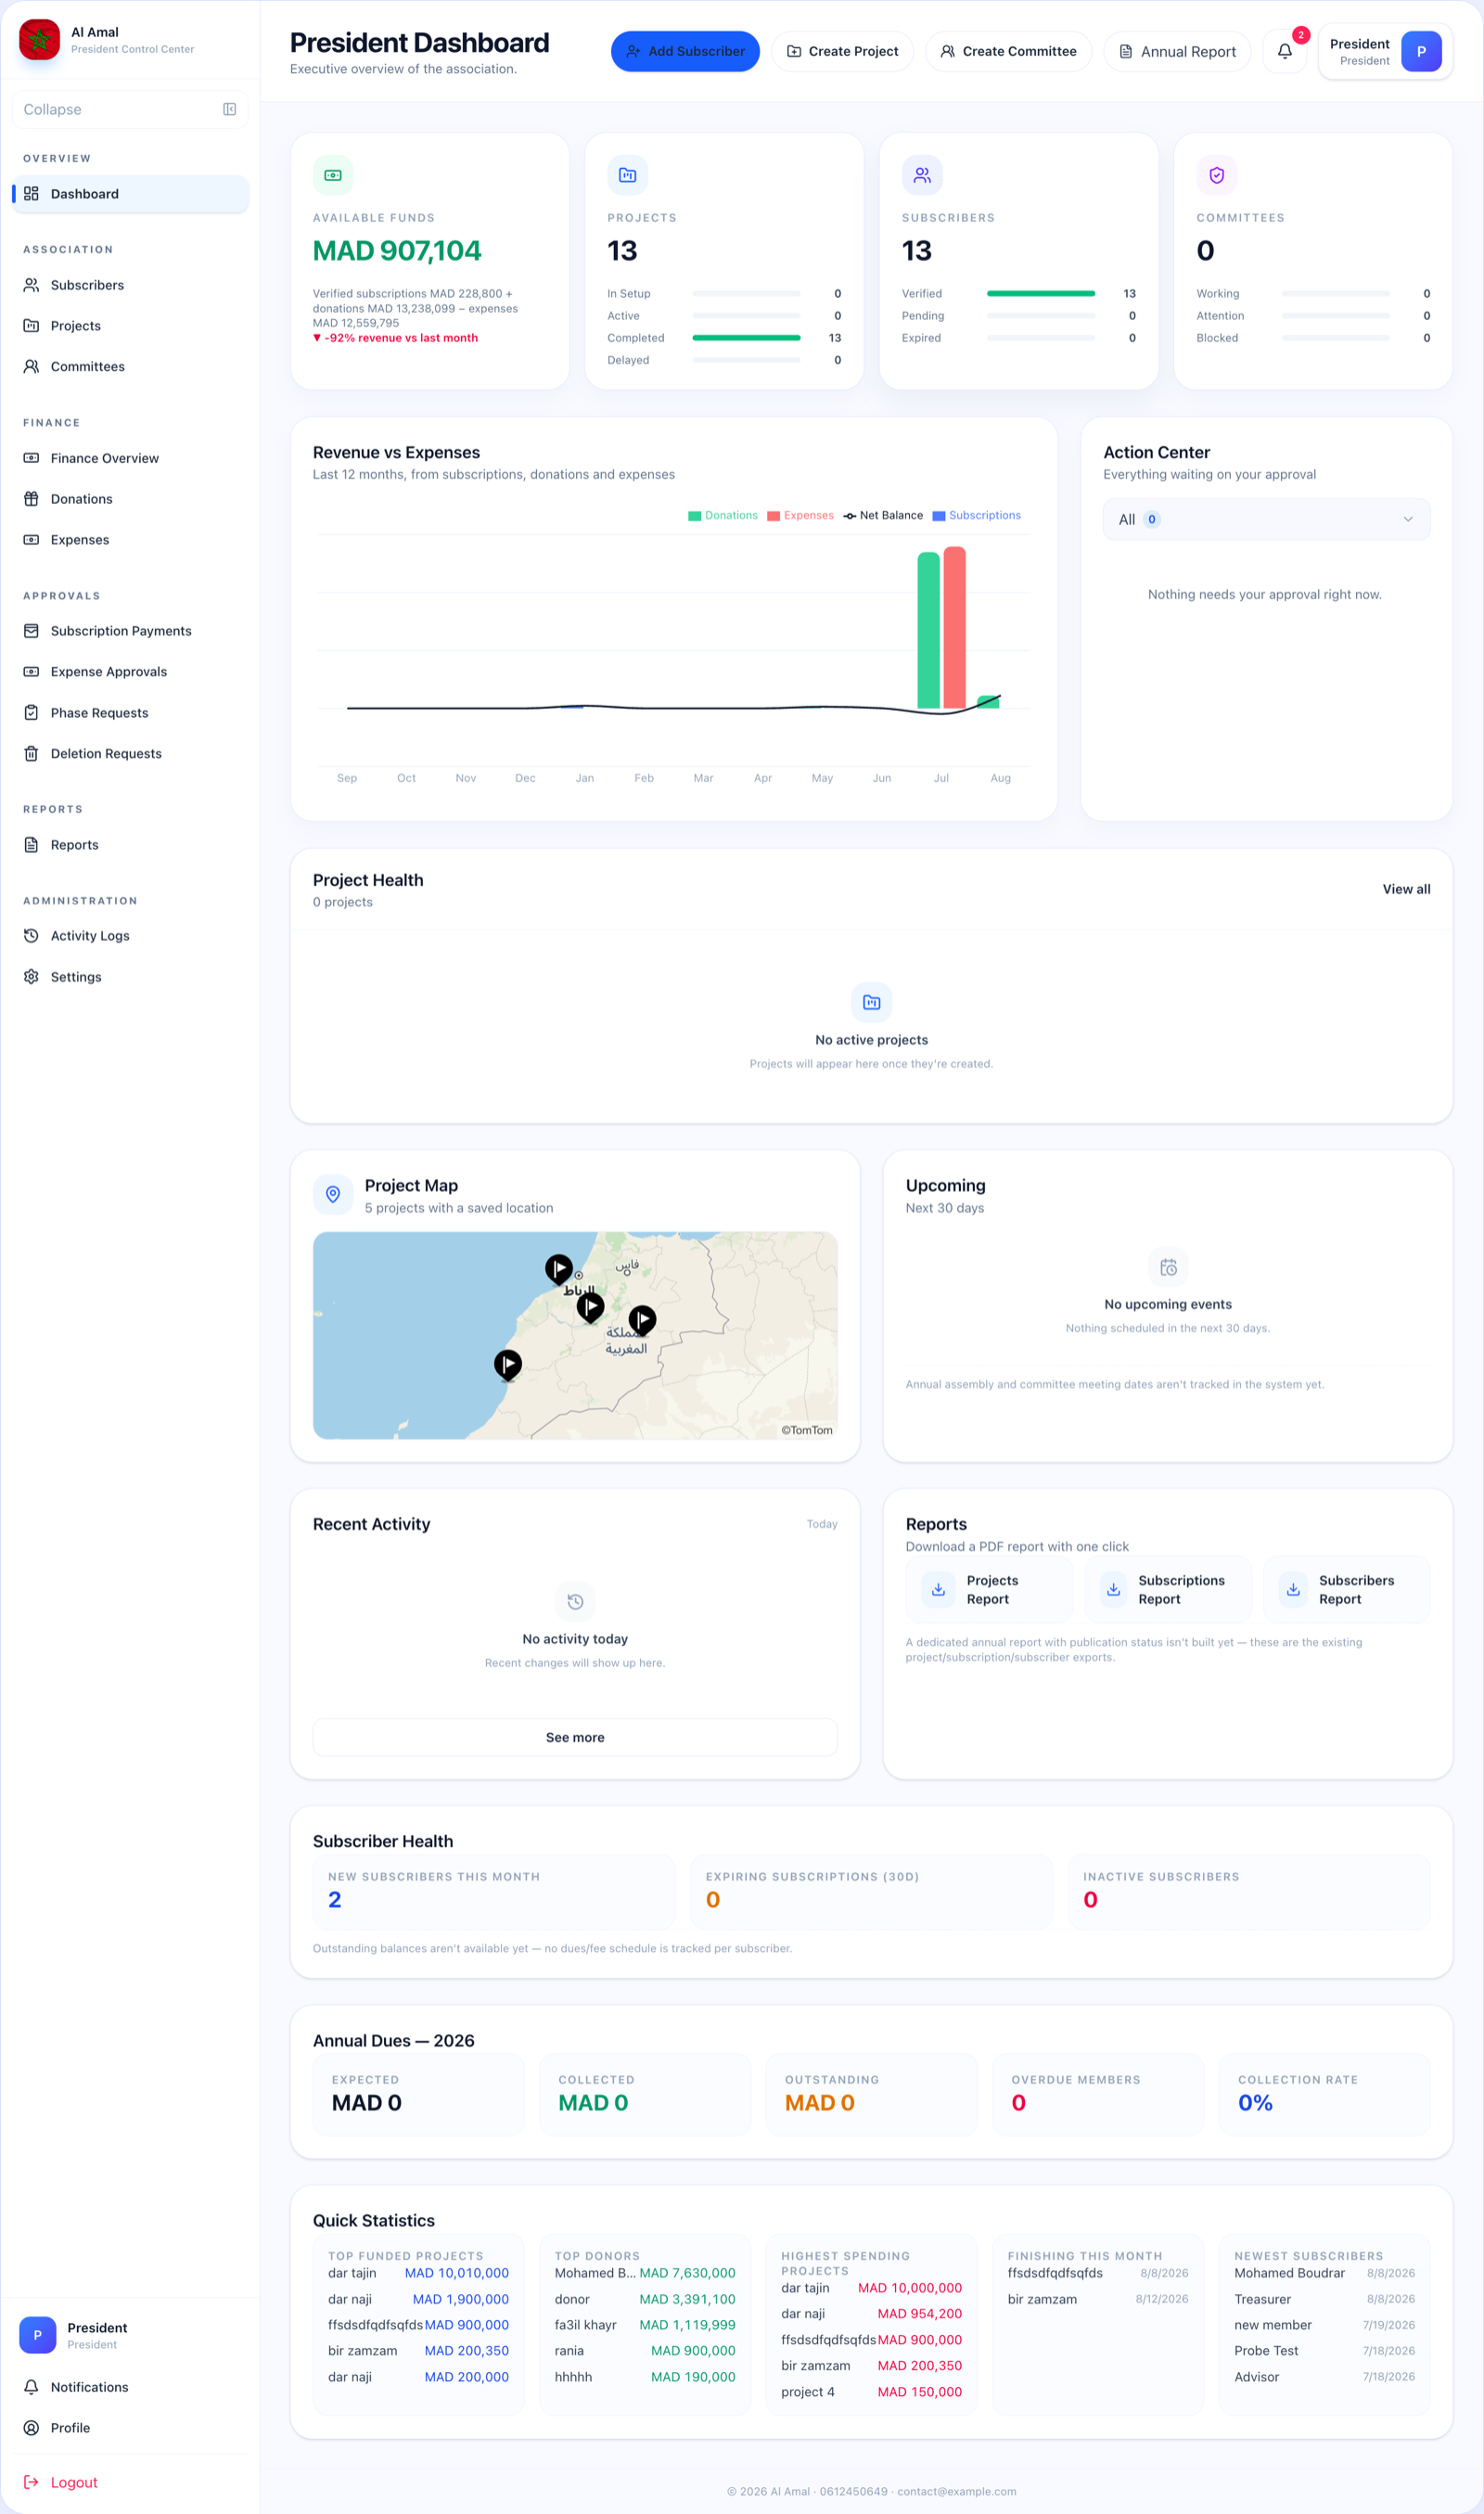
\includegraphics[width=0.92\linewidth,height=0.78\textheight,keepaspectratio]{figures/interface-dashboard.png}
  \caption{Tableau de bord du président : vue d'ensemble de l'association.}
  \label{fig:if-dashboard}
\end{figure}

\subsection{Gestion des adhérents}

Cette interface permet de créer un adhérent, de consulter et de mettre à
jour ses coordonnées, et de le supprimer.

\begin{figure}[htbp]
  \centering
  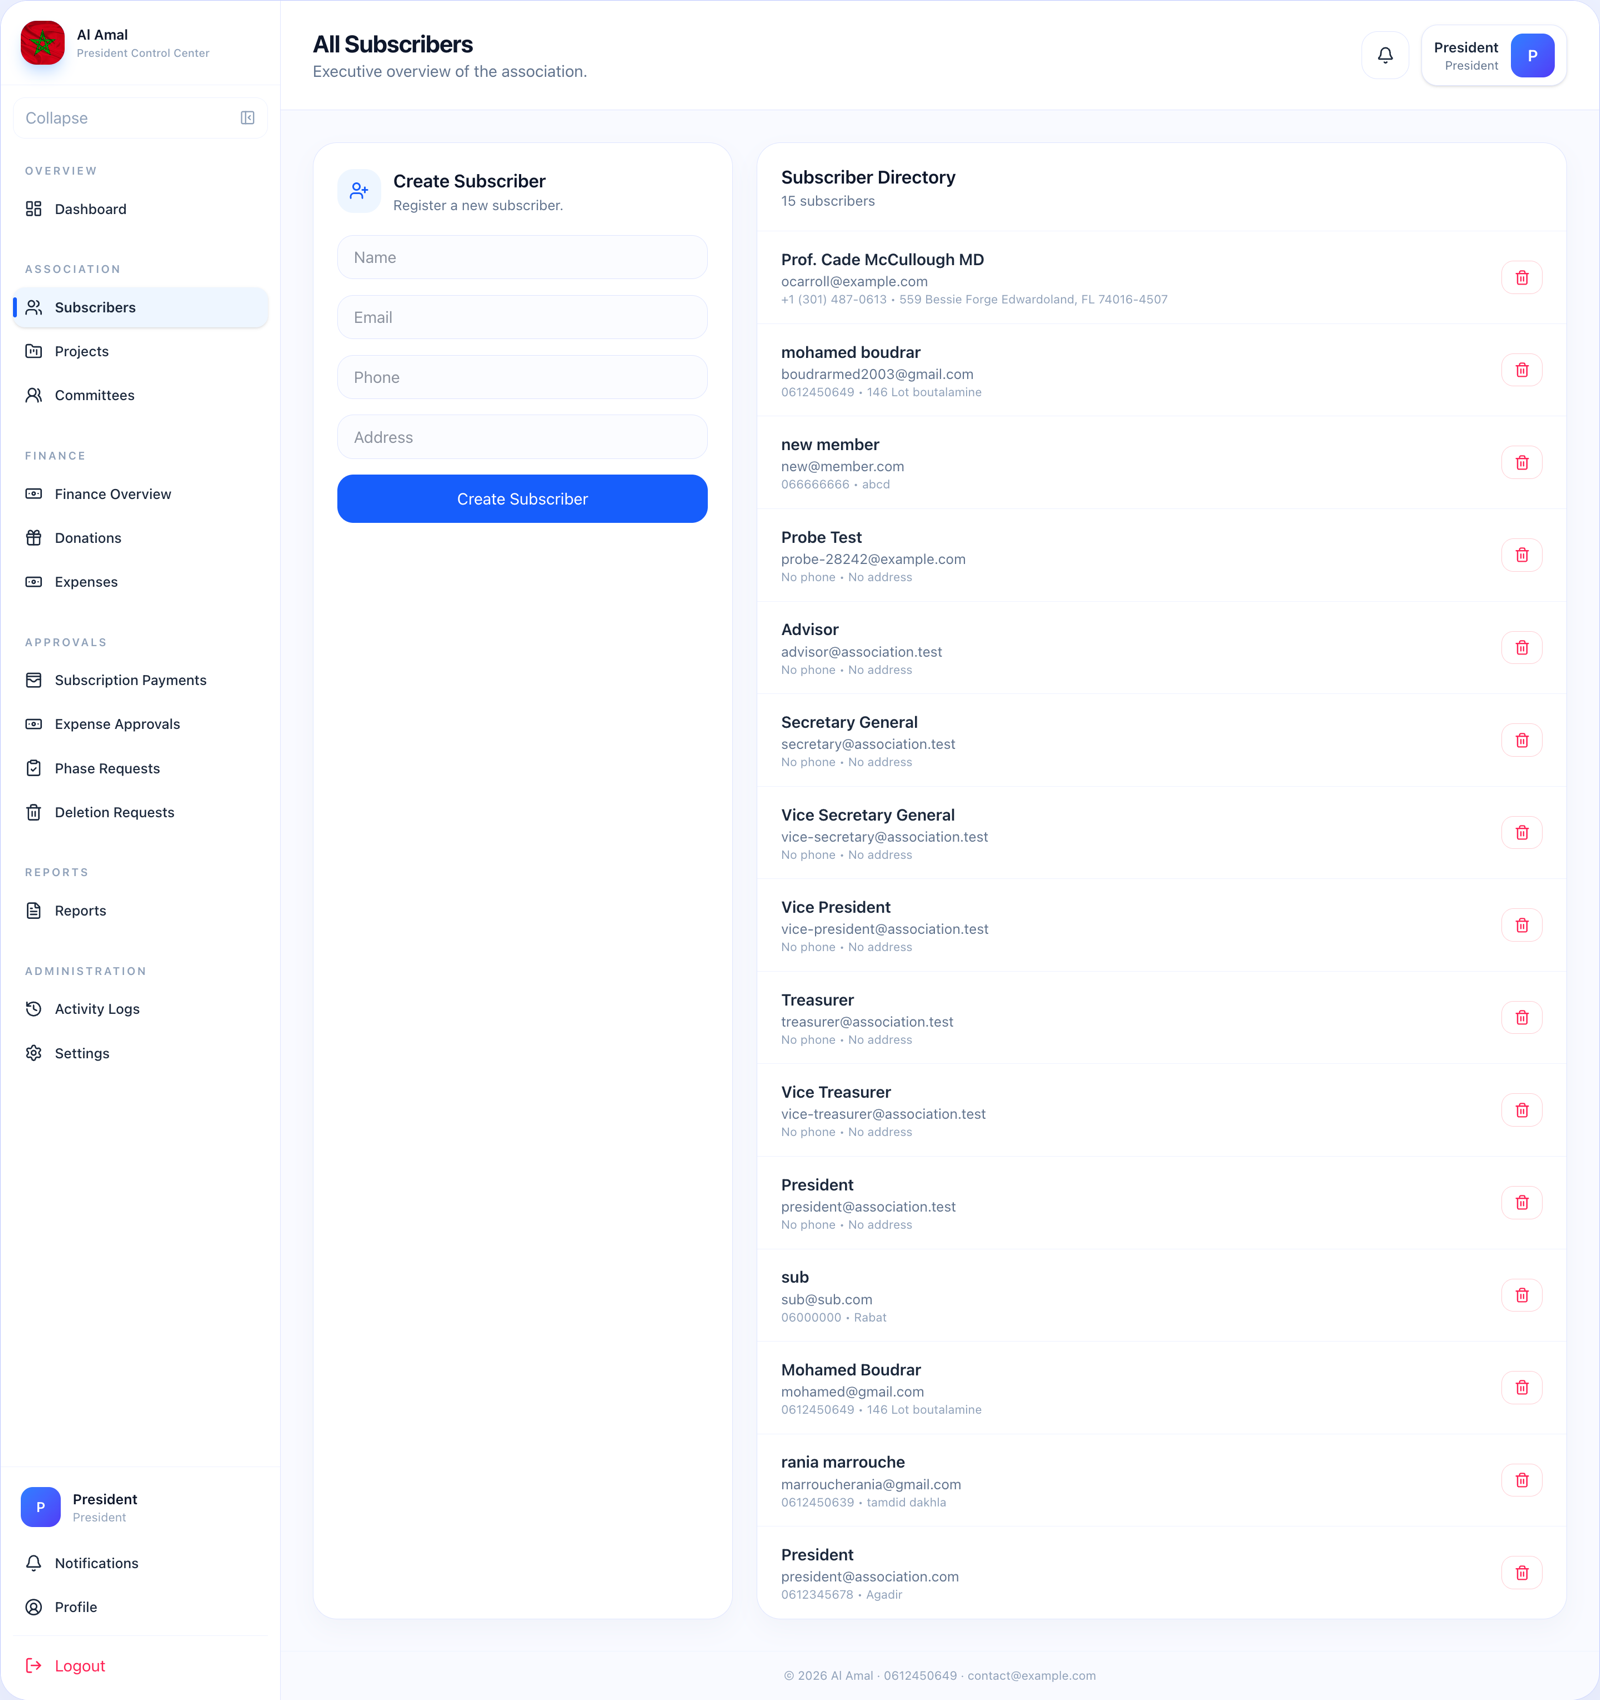
\includegraphics[width=0.92\linewidth,height=0.78\textheight,keepaspectratio]{figures/interface-membres.png}
  \caption{Gestion des adhérents.}
  \label{fig:if-membres}
\end{figure}

\subsection{Projets et comités}

La liste des projets présente leur état d'avancement ; chaque projet dispose
d'un espace de travail dédié pour son comité (figure~\ref{fig:if-projets}),
et un écran séparé permet de gérer les membres d'un comité et de consulter
son historique (figure~\ref{fig:if-comites}).

\begin{figure}[htbp]
  \centering
  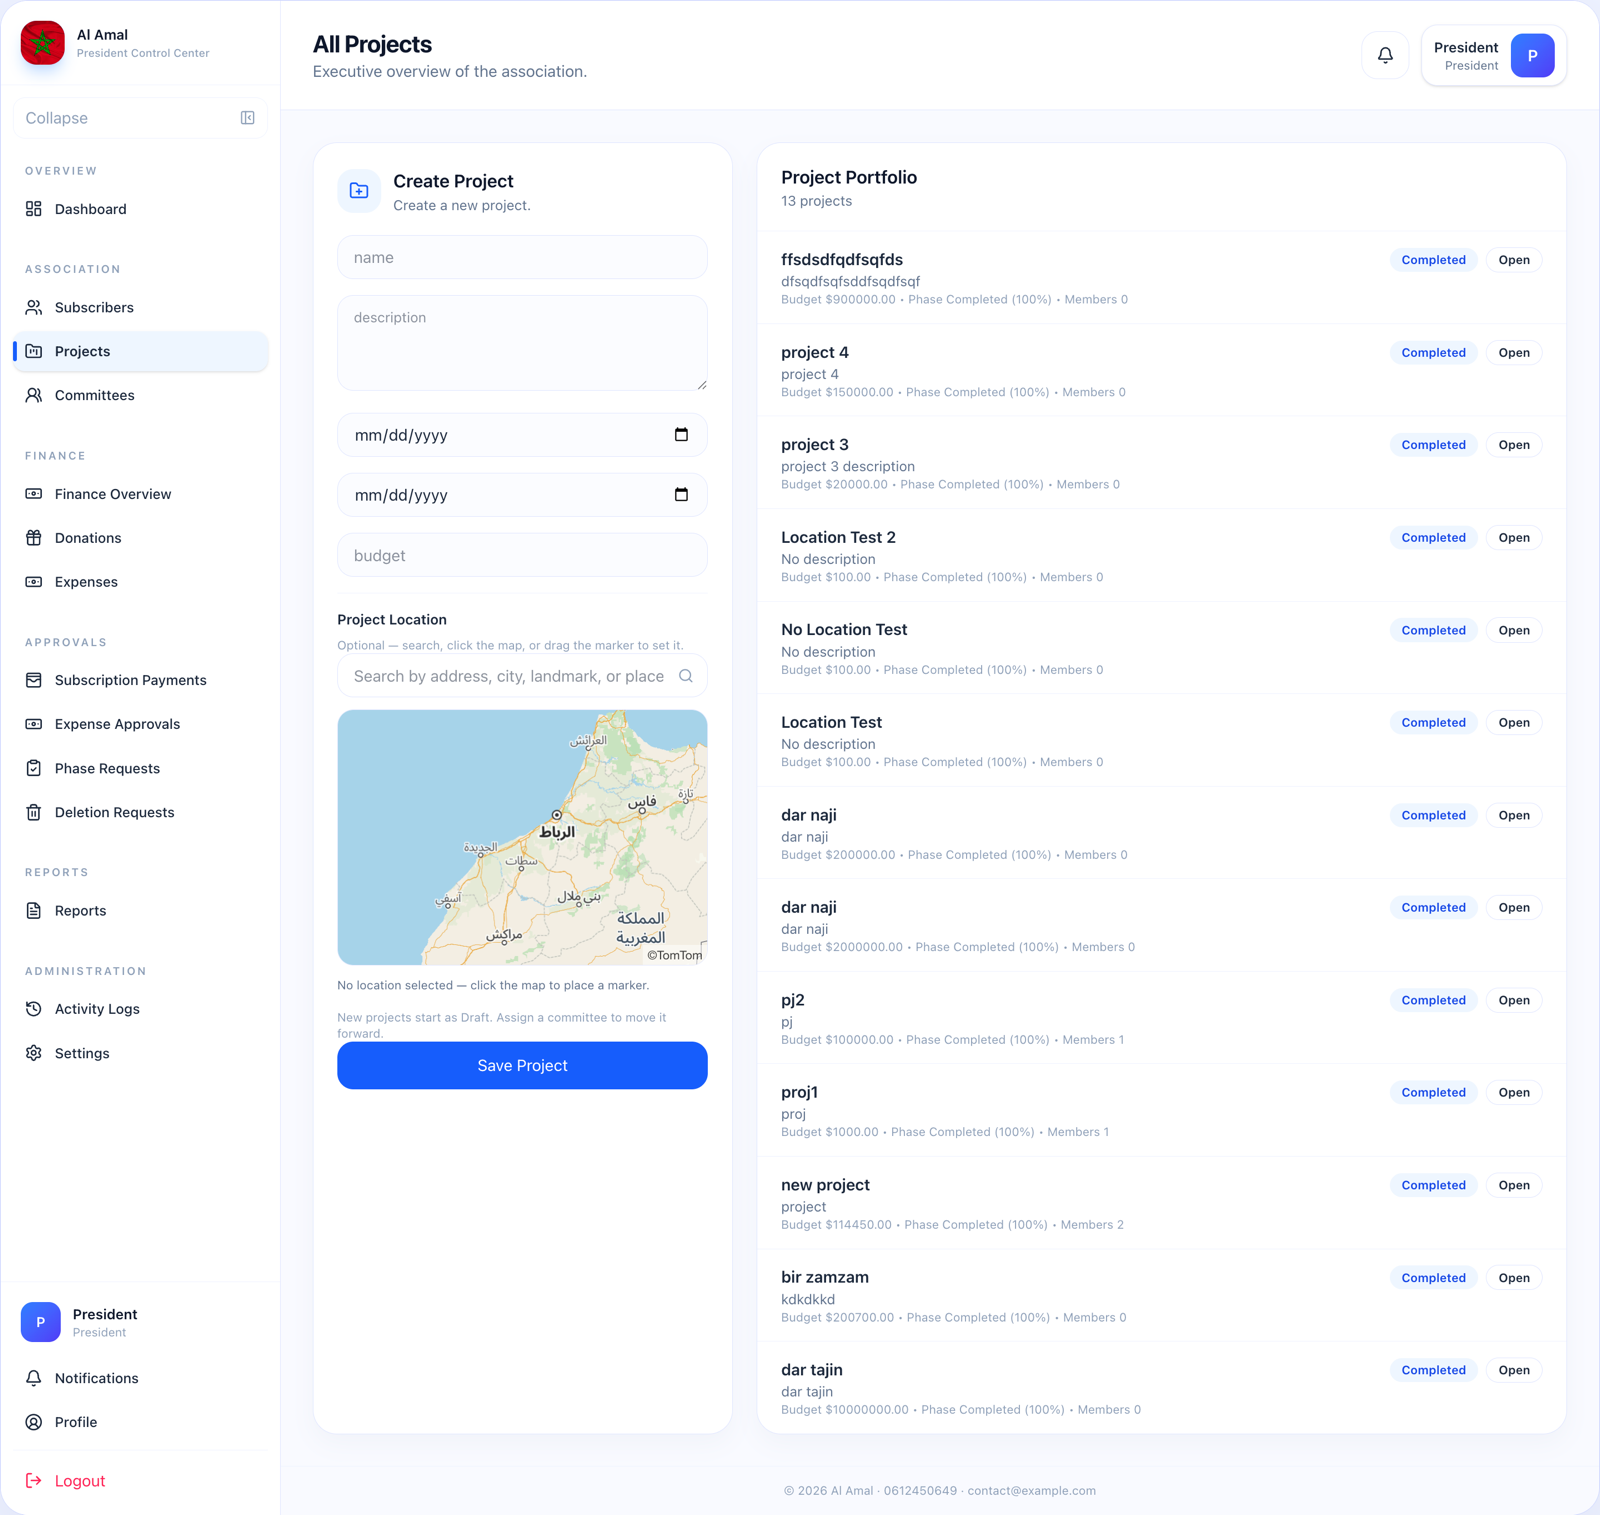
\includegraphics[width=0.92\linewidth,height=0.78\textheight,keepaspectratio]{figures/interface-projets.png}
  \caption{Liste des projets de l'association.}
  \label{fig:if-projets}
\end{figure}

\begin{figure}[htbp]
  \centering
  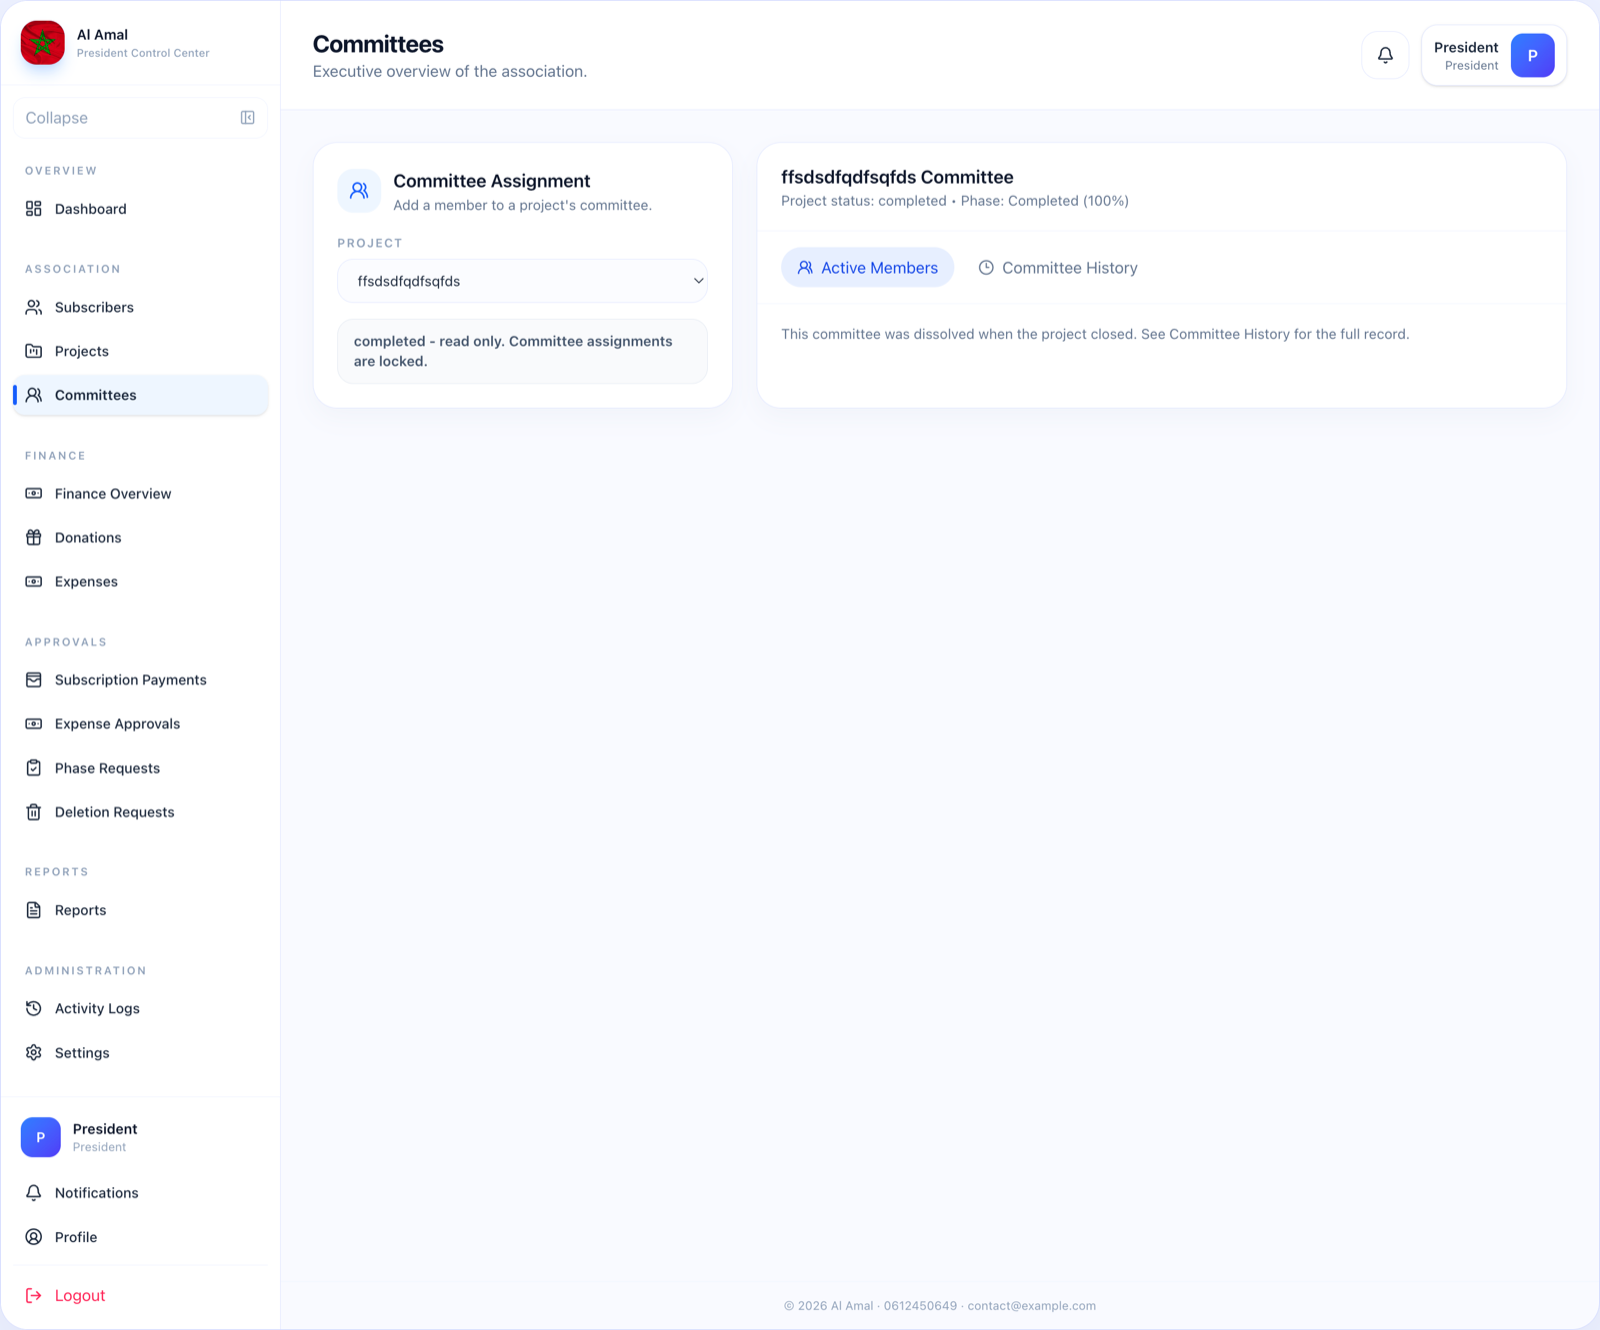
\includegraphics[width=0.92\linewidth,height=0.78\textheight,keepaspectratio]{figures/interface-comites.png}
  \caption{Gestion d'un comité de projet.}
  \label{fig:if-comites}
\end{figure}

\subsection{Finances}

L'écran des finances présente les fonds disponibles, les dons regroupés par
projet, et le financement de chaque projet (budget, dons, alloué, dépenses,
solde restant).

\begin{figure}[htbp]
  \centering
  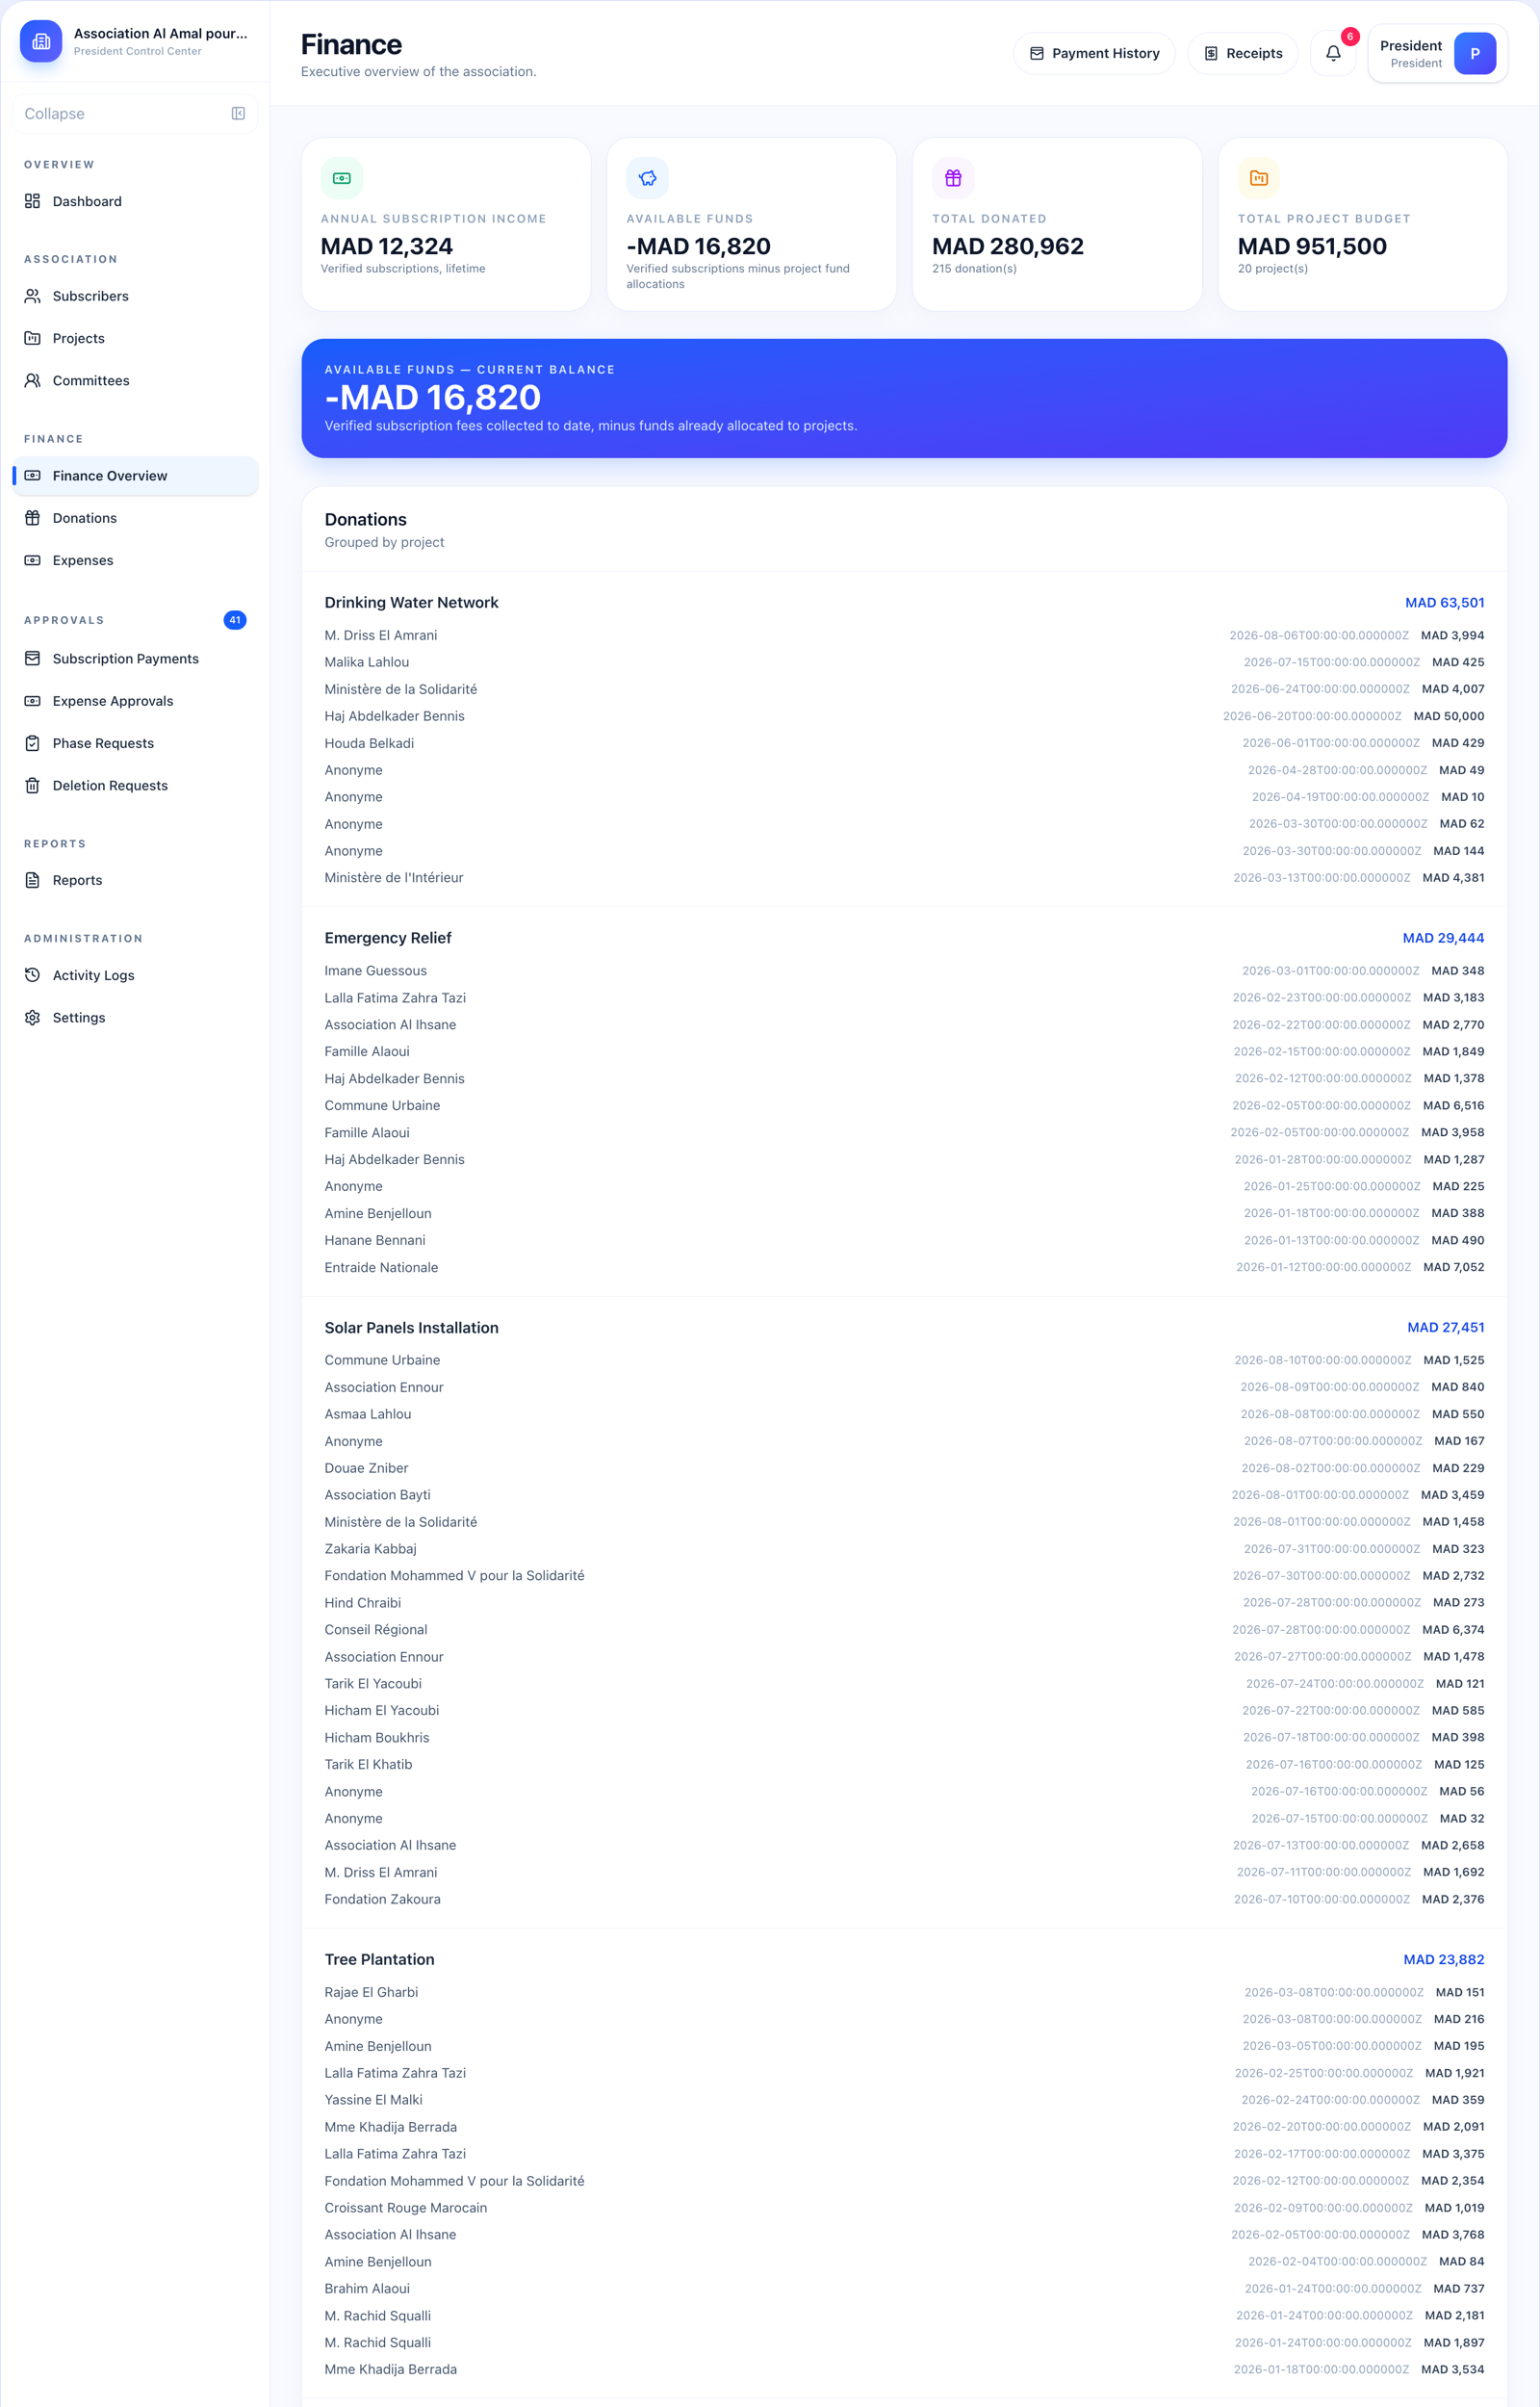
\includegraphics[width=0.92\linewidth,height=0.78\textheight,keepaspectratio]{figures/interface-finances.png}
  \caption{Vue d'ensemble des finances de l'association.}
  \label{fig:if-finances}
\end{figure}

\subsection{Approbations}

Les files d'approbation (cotisations, dons, dépenses, demandes de passage de
phase, demandes de suppression de projet) regroupent tout ce qui attend une
décision d'un rôle habilité.

\begin{figure}[htbp]
  \centering
  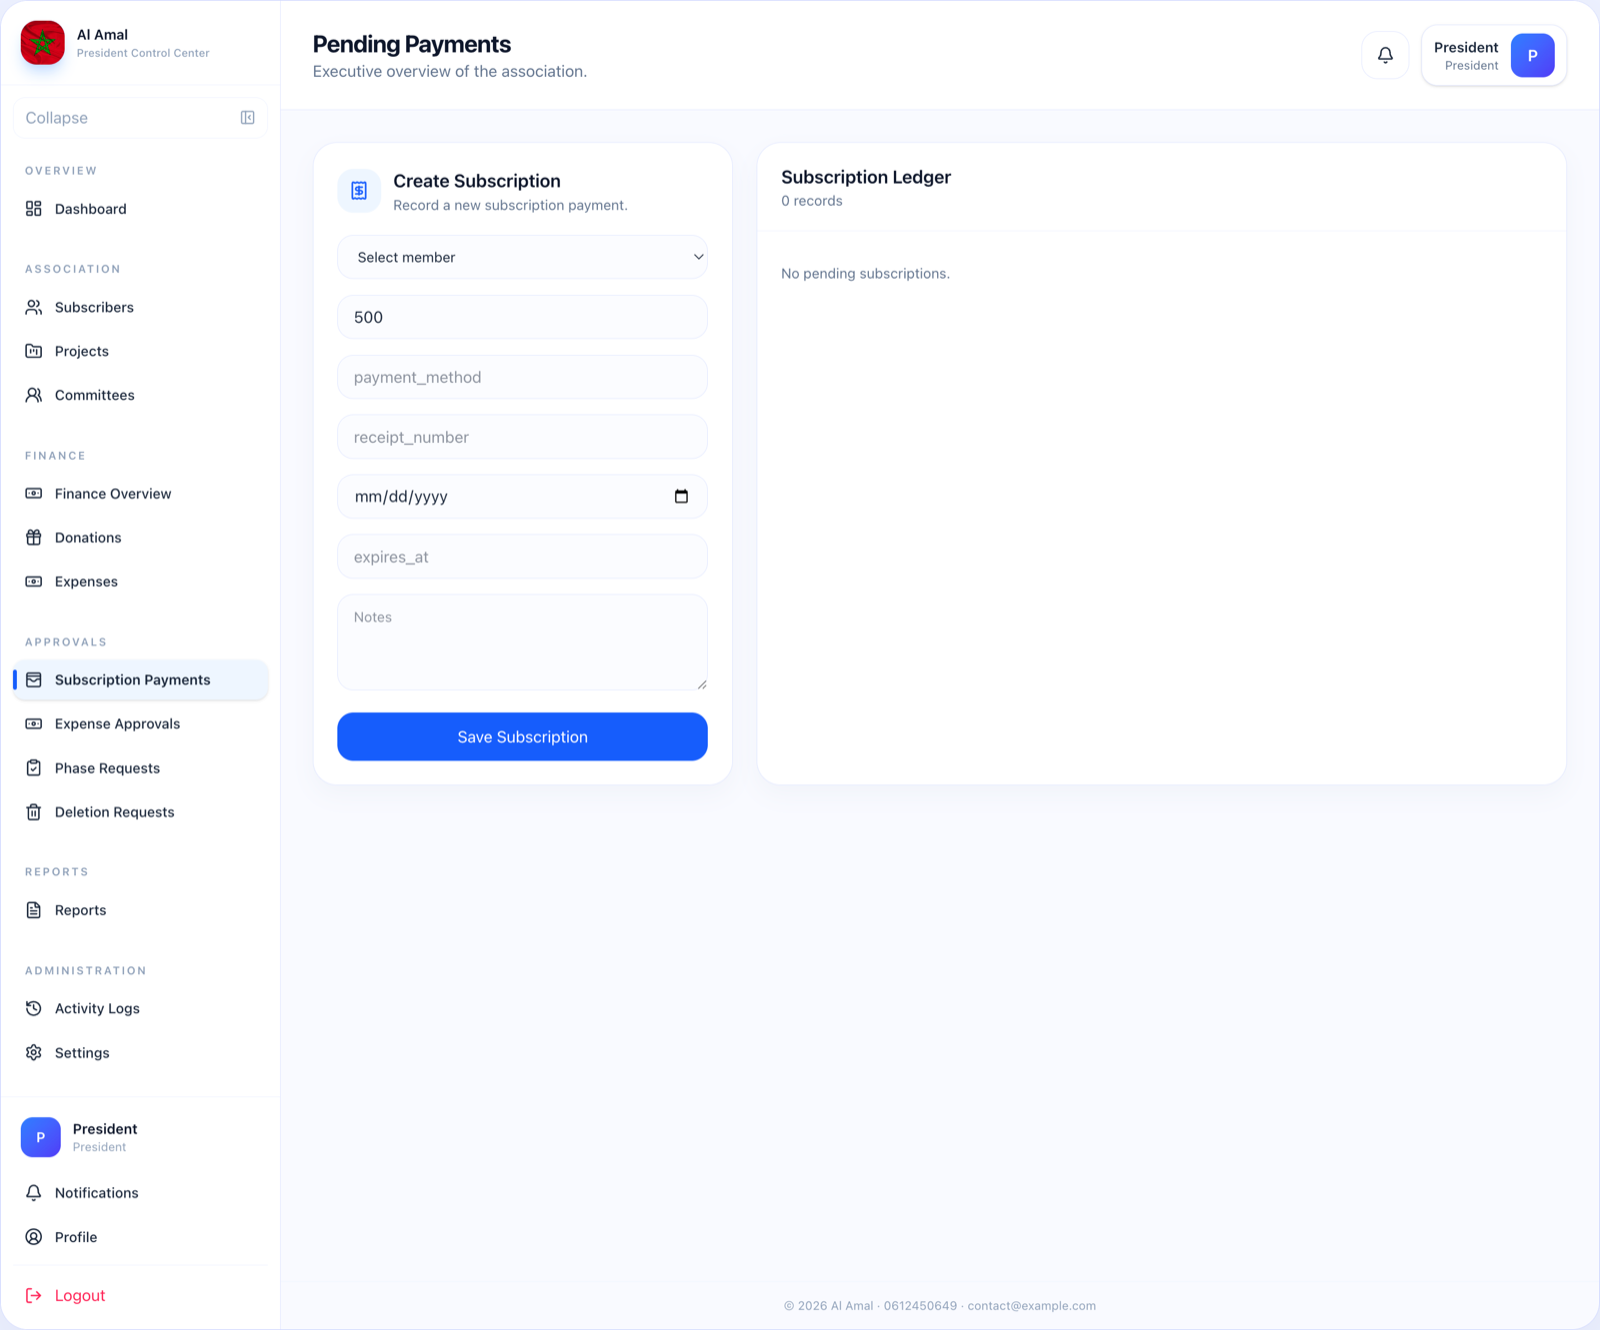
\includegraphics[width=0.92\linewidth,height=0.78\textheight,keepaspectratio]{figures/interface-approbations.png}
  \caption{File d'attente des cotisations à vérifier.}
  \label{fig:if-approbations}
\end{figure}

\subsection{Rapports}

Cet écran centralise le téléchargement des rapports association (adhérents,
cotisations, projets, cotisations dues) en PDF ou en Excel.

\begin{figure}[htbp]
  \centering
  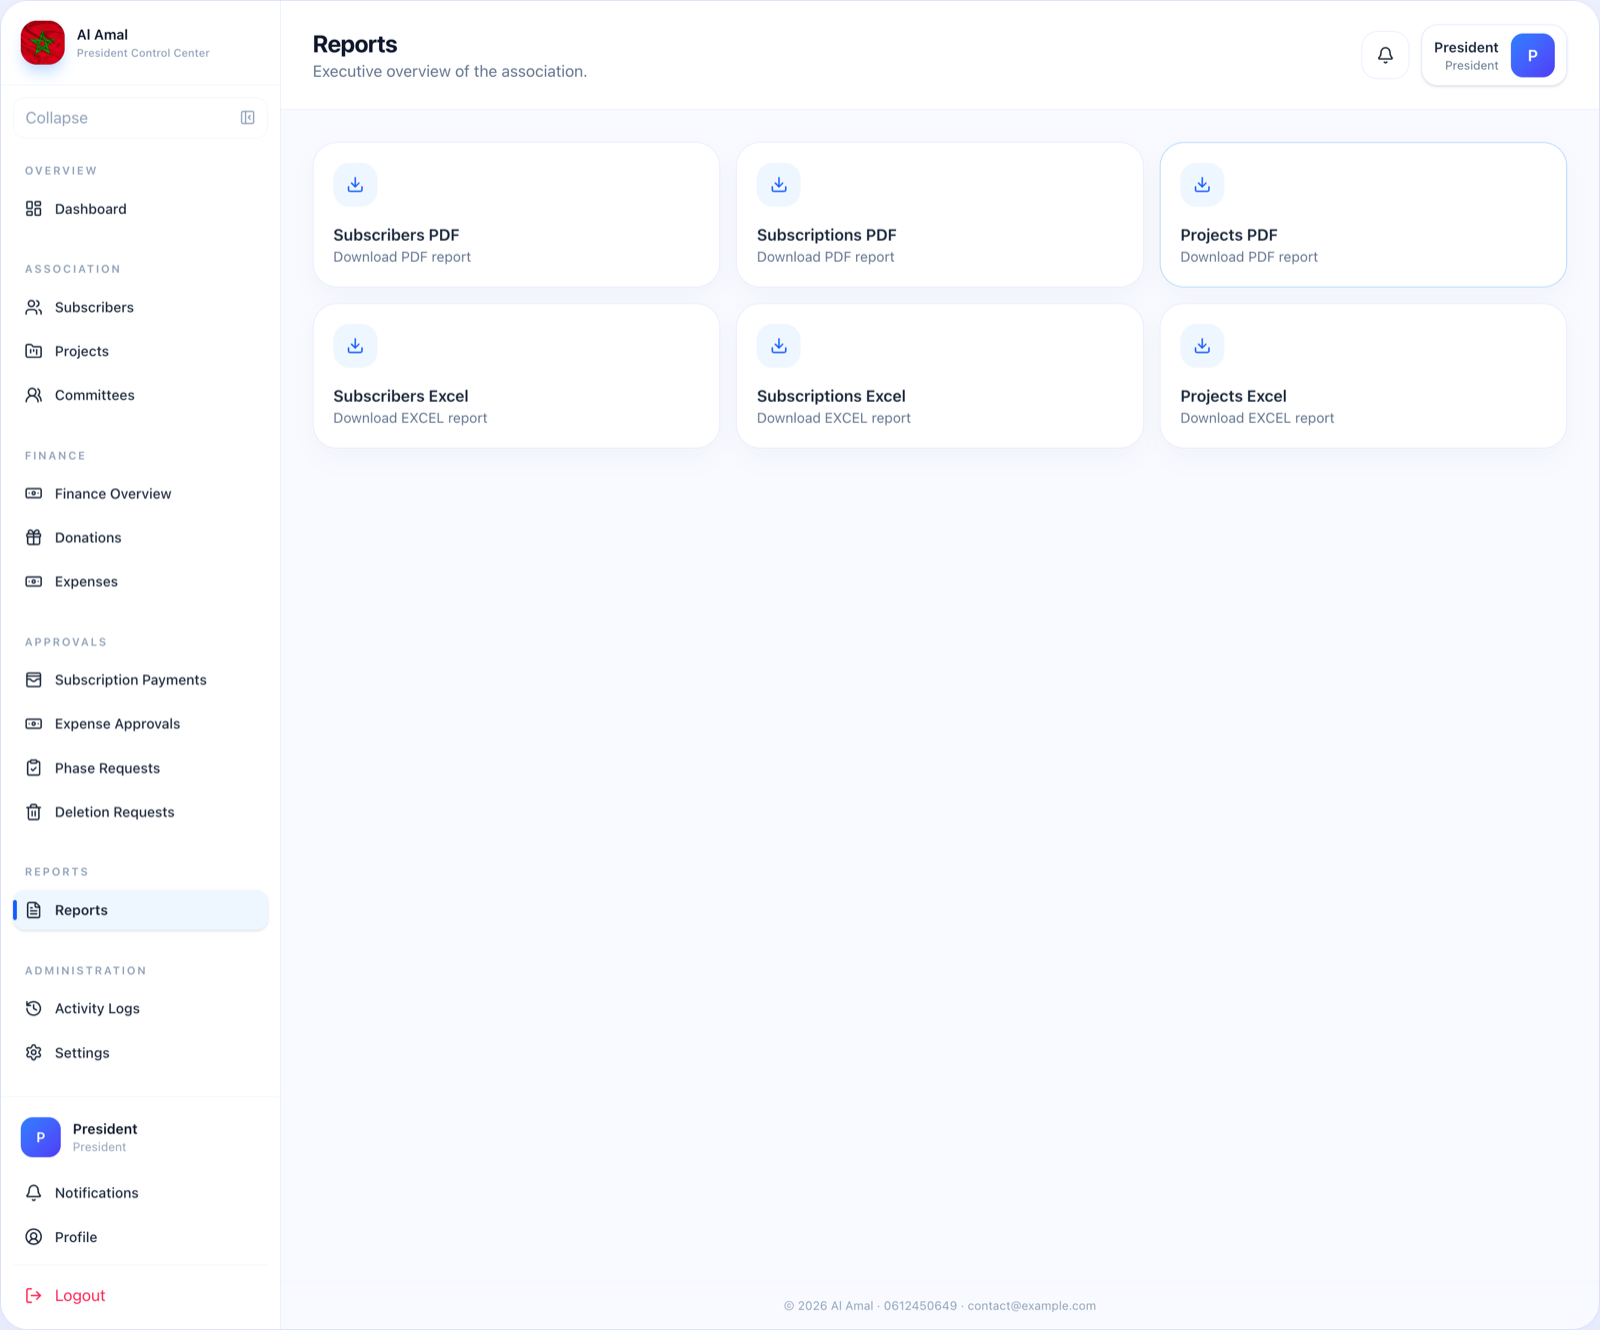
\includegraphics[width=0.92\linewidth,height=0.78\textheight,keepaspectratio]{figures/interface-rapports.png}
  \caption{Écran des rapports association.}
  \label{fig:if-rapports}
\end{figure}

\subsection{Paramètres}

Réservé au président, cet écran configure l'identité de l'association (nom,
logo, coordonnées) et le montant de la cotisation annuelle par défaut.

\begin{figure}[htbp]
  \centering
  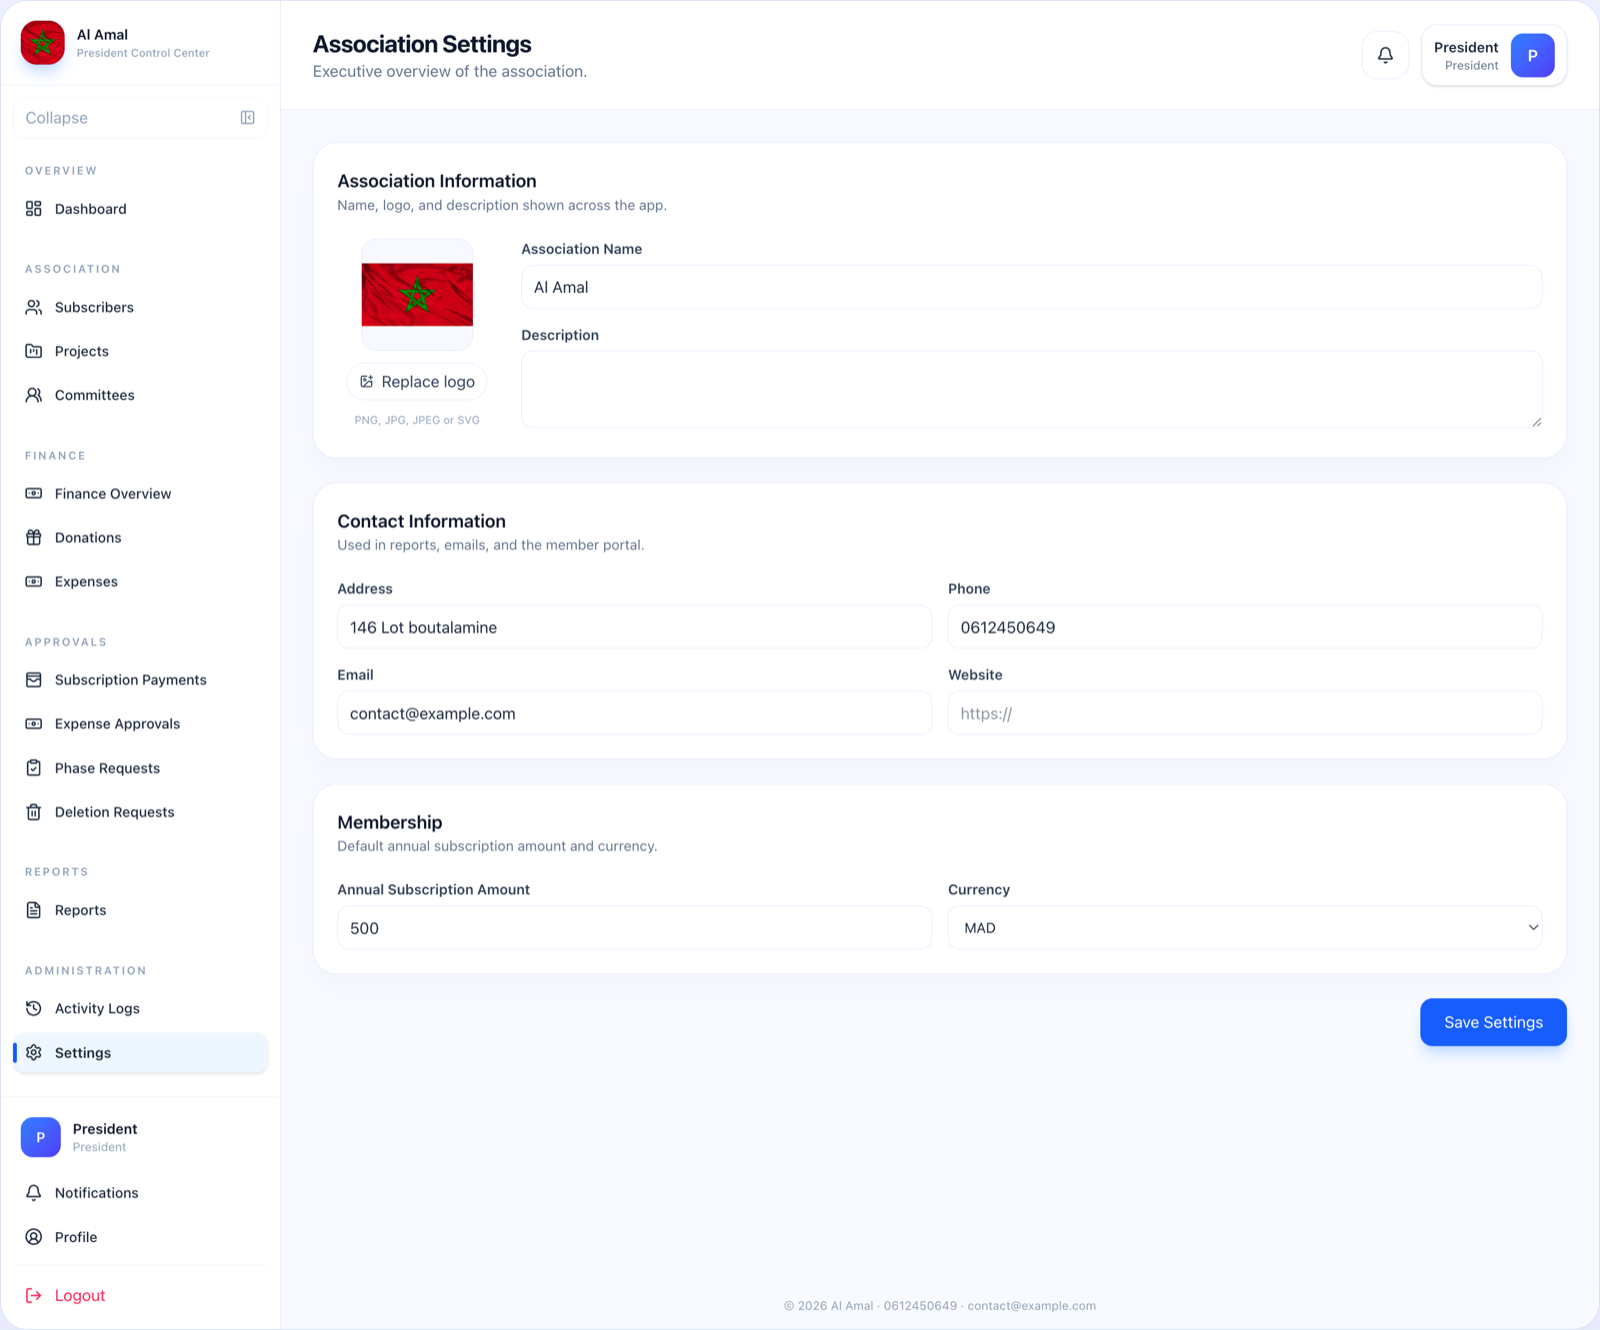
\includegraphics[width=0.92\linewidth,height=0.78\textheight,keepaspectratio]{figures/interface-parametres.png}
  \caption{Paramètres de l'association.}
  \label{fig:if-parametres}
\end{figure}

\section{Conclusion}

Ce chapitre a présenté la spécification fonctionnelle, les acteurs du système
et la structure conceptuelle des données, ainsi que l'architecture technique
retenue, l'environnement de développement, les fonctionnalités implémentées
et les interfaces développées pour chaque profil d'utilisateur.
